\section{\Large PROBLEM SET 4}
\subsection{PROBLEM 1}
\textit{Equilibrium tests}

\textit{a. Assume that 2 components of the initial angular velocities are zero and that the principal axes are aligned with the inertial frame (e.g., zero Euler angles). Verify that during the simulation the 2 components of angular velocity remain zero and that the attitude represents a pure rotation about the rotation axis (e.g., linearly increasing Euler angle). Plot velocities and angles.}

To test the equilibrium state, we choose the following initial angular velocity,

\begin{align*}
\Vec{\omega} &= 
\qty[parse-numbers = false]{
    \begin{bmatrix}
    0 \\
    0 \\
    1 \\ 
    \end{bmatrix}
}{\radian\per\s},
\end{align*}

and we set all Euler angles to zero. We use a 312 convention for Euler angles, which avoids singularities for this configuration.

Figure \ref{fig:ps4_problem1a_angvel} shows results of the simulation, where $\omega_x$ and $\omega_y$ remain zero and $\omega_z$ maintains a constant value.

\begin{figure}[H]
\centering
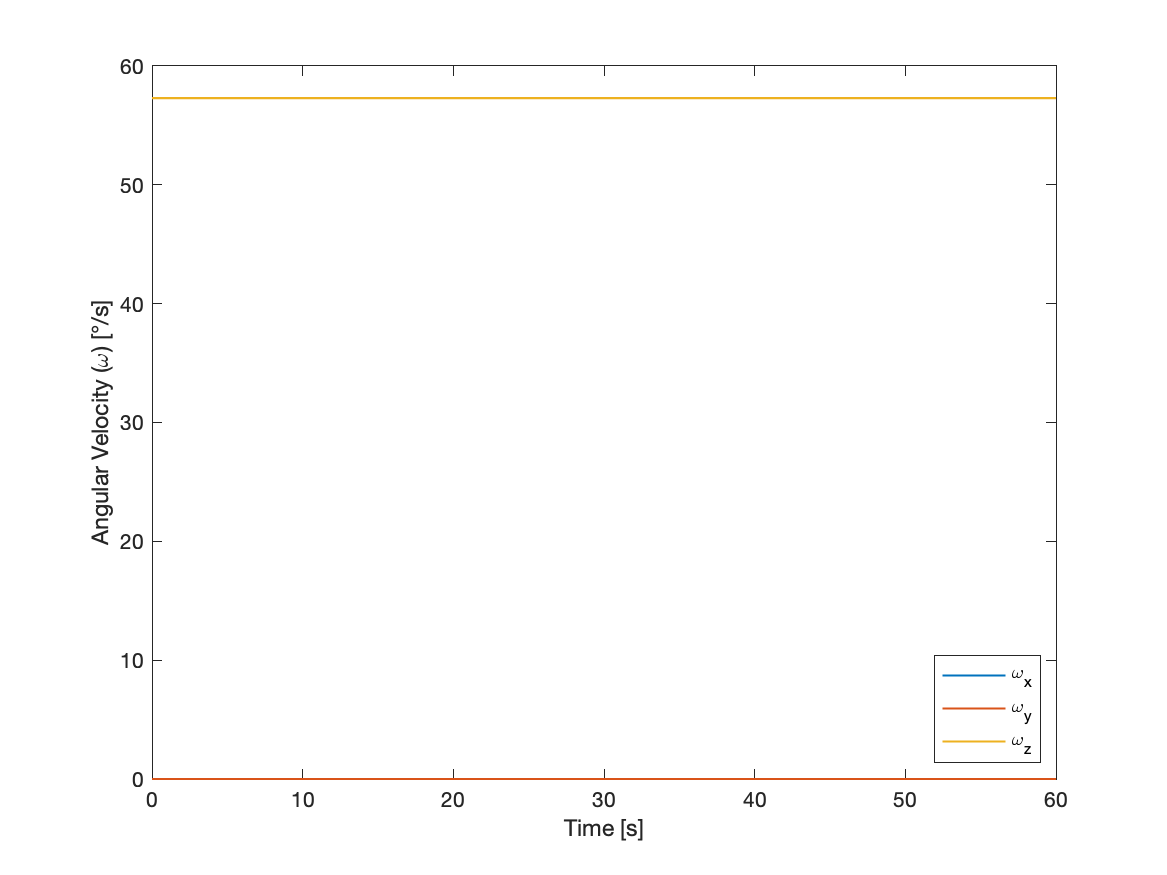
\includegraphics[scale=0.6]{Images/ps4_problem1a_angvel.png}
\caption{Evolution of angular velocity}
\label{fig:ps4_problem1a_angvel}
\end{figure}

Similarly, in Figure \ref{fig:ps4_problem1a_angle}, $\phi$ and $\theta$ Euler angles remain at zero while the $\psi$ Euler angle increases linearly.

\begin{figure}[H]
\centering
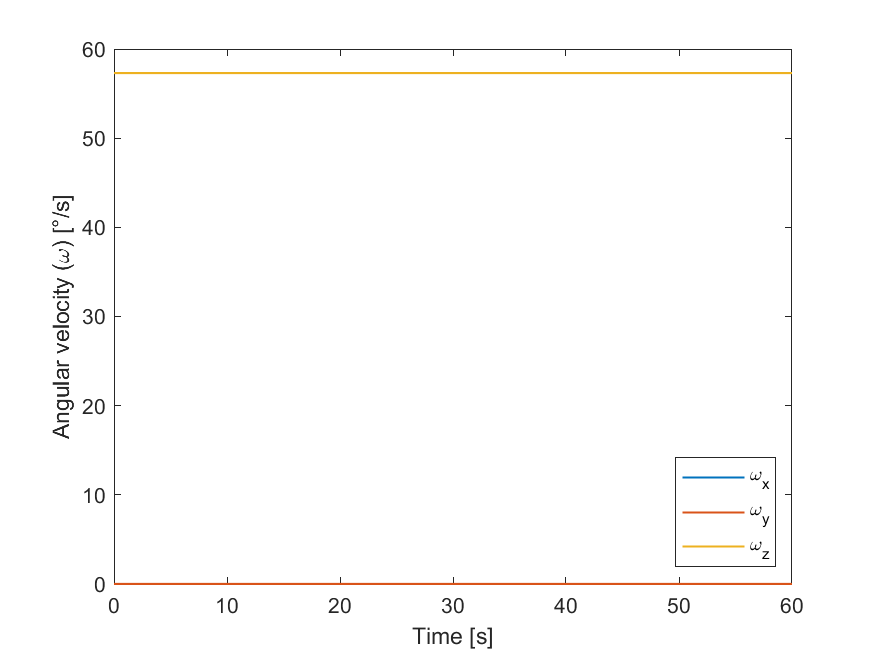
\includegraphics[scale=0.6]{Images/ps4_problem1a_angle.png}
\caption{Evolution of Euler angles}
\label{fig:ps4_problem1a_angle}
\end{figure}

\textit{b. Repeat a. by setting the initial attitude to match the RTN frame. Set the initial angular velocity to be non-zero only about N. Show the evolution of attitude motion in the RTN frame and give an interpretation of the results (recall that you might have J2 effects in orbit propagation, consider removing them for verification).}

We choose to align our principal axes with the RTN frame. For selected initial orbital conditions taken from the NISAR science users' handbook, we obtain the initial position and compute the RTN frame, which we then use to find initial aligned Euler angles.

\begin{figure}[H]
\centering
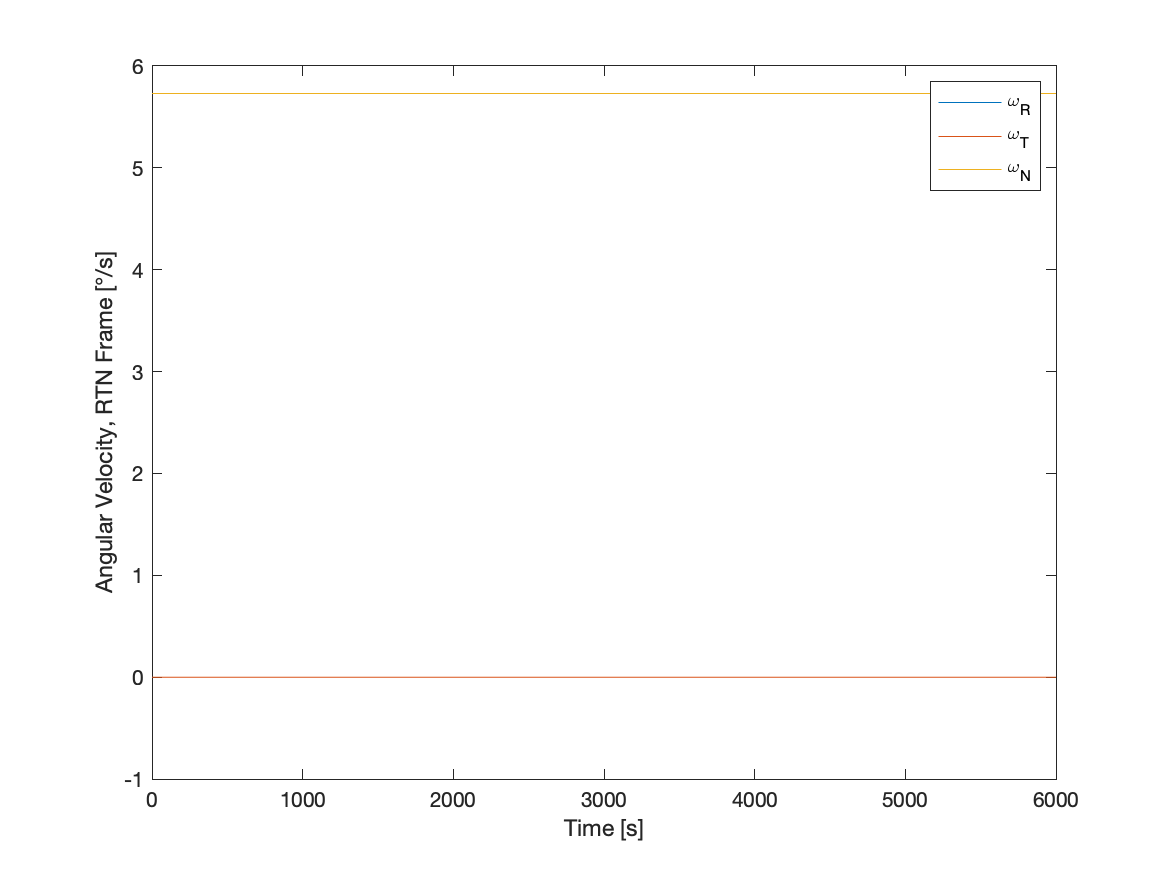
\includegraphics[scale=0.6]{Images/ps4_problem1b_angvel.png}
\caption{Evolution of angular velocity}
\label{fig:ps4_problem1b_angvel}
\end{figure}

We set a nonzero $\omega_z$ angular velocity, which is aligned with the normal direction of the RTN frame, and we choose all other angular velocities to be zero. Propagating the orbit and attitude, we find that the angular velocity remains constant throughout the orbit, even relative to the RTN frame, as seen in Figure \ref{fig:ps4_problem1b_angvel}. From Figure \ref{fig:ps4_problem1b_euler}, we see that the $\theta$ and $\psi$ Euler angles related to the RTN frame are constant while $\phi$ varies.

\begin{figure}[H]
\centering
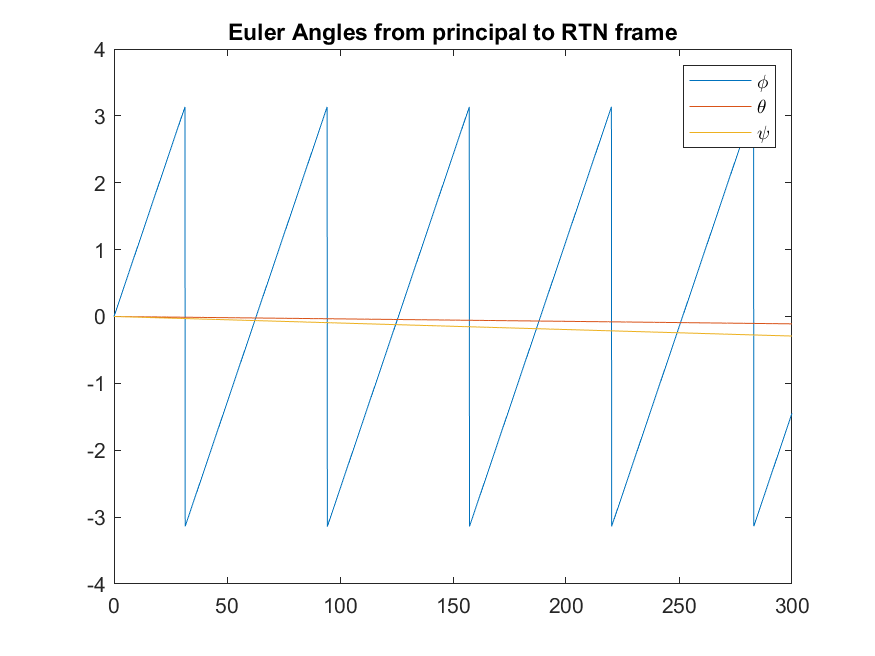
\includegraphics[scale=0.6]{Images/ps4_problem1b_euler.png}
\caption{Evolution of Euler angles}
\label{fig:ps4_problem1b_euler}
\end{figure}

This result shows our satellite's maximum inertia principal axis remains aligned with the normal direction of the orbit such that the maximum inertia principal axis remains normal to the plane of the orbit, given the initial condition that axes are aligned with the RTN frame and angular velocity along other axes is nonzero.

\subsection{PROBLEM 2}
\textit{Stability tests}

\textit{a. Pretend you have a single-spin satellite. Set initial conditions to correspond alternatively to the 3 possible equilibrium configurations (rotation about principal axes of inertia). Slightly perturb initial condition. Is the attitude stable or unstable? In angles and velocities? If stable, periodically or asymptotically? Show it.}

For a single spin satellite, the three possible equilibrium configurations are rotation about the minimum inertia principal axis, rotation about the intermediate axis, and rotation about the maximum inertia principal axis. Figures \ref{fig:ps4_problem2a_1}, \ref{fig:ps4_problem2a_2}, \ref{fig:ps4_problem2a_3} show that the Euler angles are stable about the minimum and maximum axes, but it is unstable about the intermediate axes. This is as expected for our system, with the minimum and maximum axes exhibiting periodic stability with small oscillations in angular velocity.

\begin{figure}[H]
\centering
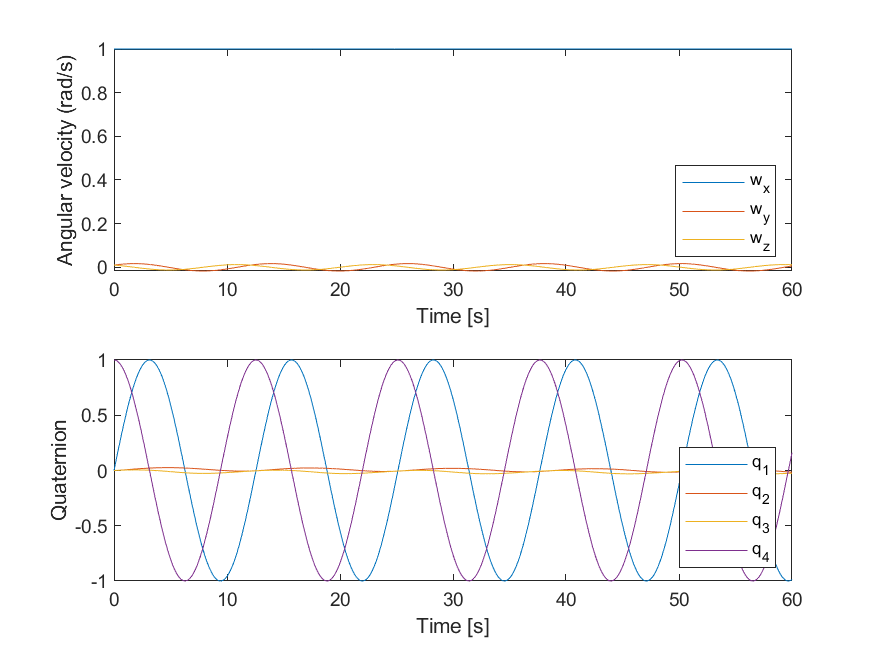
\includegraphics[scale=0.6]{Images/ps4_problem2a_1.png}
\caption{Simulation of satellite spinning on its minimum principal axis}
\label{fig:ps4_problem2a_1}
\end{figure}

Note that while in Figure \ref{fig:ps4_problem2a_1} the angular velocities are periodically stable, the Euler angles oscillate. This is likely a consequence of the sequence of rotations used for our choice of Euler angle convention.

\begin{figure}[H]
\centering
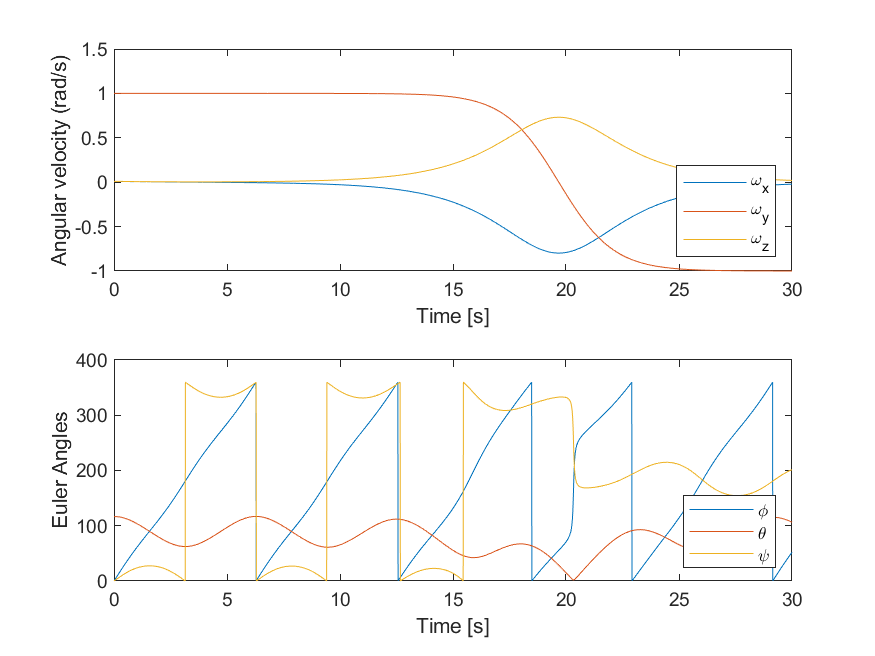
\includegraphics[scale=0.6]{Images/ps4_problem2a_2.png}
\caption{Simulation of satellite spinning on its intermediate principal axis}
\label{fig:ps4_problem2a_2}
\end{figure}

\begin{figure}[H]
\centering
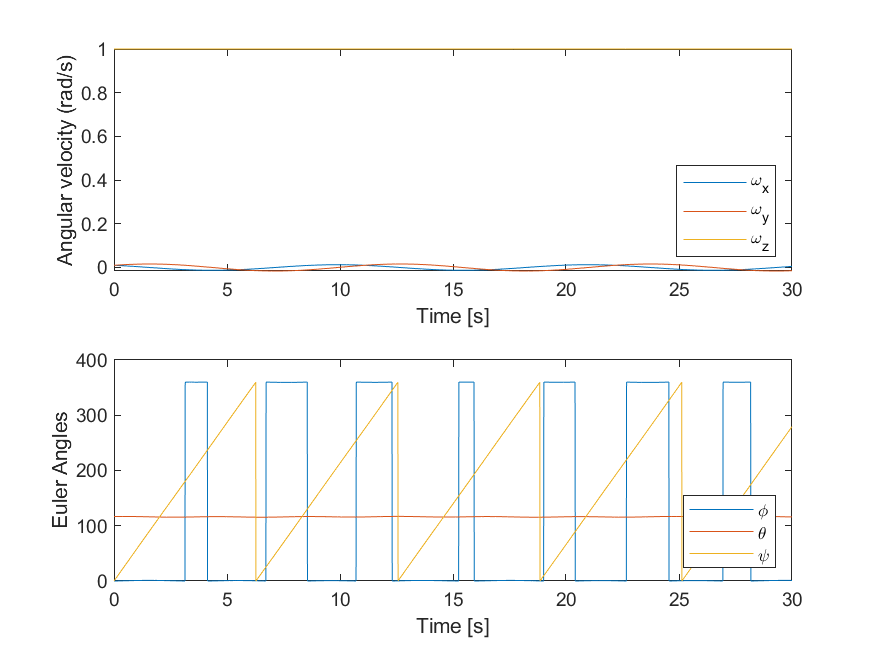
\includegraphics[scale=0.6]{Images/ps4_problem2a_3.png}
\caption{Simulation of satellite spinning on its maximum principal axis}
\label{fig:ps4_problem2a_3}
\end{figure}

\subsection{PROBLEM 3}
\textit{Adding a momentum wheel or rotor (dual-spin satellite)}

\textit{a. Re-program Euler equations to include a generic momentum wheel or rotor with rotation axis aligned with one of the principal axes of inertia. Ideally the wheel or rotor has specs representative of commercial products (inertia, rotational speed).}

We choose to use specifications from the RSI 68 momentum wheel, for which datasheets are readily available online \cite{RSI68}. This particular momentum wheel is intended for spacecraft in the 1,500 to 5,000 kg range, which matches our mission. We use a diameter of 347 mm and mass of 8.9 kg and model our reaction wheel as a hoop with mass concentrated about the outer diameter. We also use 2,500 RPM, which yields approximately the nominal angular momentum from the datasheet–the maximum angular velocity is 6,000 RPM. The following Euler equations are used to model a momentum wheel as a rotor. For this problem, we set the torques on the right side of each equation to zero, as we are not considering external torques.

\begin{align*}
    I_x \dot{\omega_x} + I_r \dot{\omega_r} r_x + (I_z - I_y) \omega_y \omega_z 
    + I_r \omega_r (\omega_y r_z - \omega_z r_y) = M_x \\
    I_y \dot{\omega_y} + I_r \dot{\omega_r} r_y + (I_x - I_z) \omega_z \omega_x 
    + I_r \omega_r (\omega_z r_x - \omega_x r_z) = M_y \\
    I_z \dot{\omega_z} + I_r \dot{\omega_r} r_z + (I_y - I_x) \omega_x \omega_y 
    + I_r \omega_r (\omega_x r_y - \omega_y r_x) = M_z \\
    I_r \dot{\omega_r} = M_r
\end{align*}

The function \texttt{kinEulerAngleWheel}, shown below, is used in addition to \texttt{ode113} to simulate the angular velocities over time.

\lstinputlisting{src/kinEulerAngleWheel.m}

\textit{b. Numerically integrate Euler AND Kinematic equations from equilibrium initial condition. Verify that integration is correct as from previous tests (conservation laws, rotations, etc.).}

Simulating the Euler and kinematic equations, Figure \ref{fig:ps4_problem3b} shows the angular momentum vector remain constant in the inertial frame, as expected.

\begin{figure}[H]
\centering
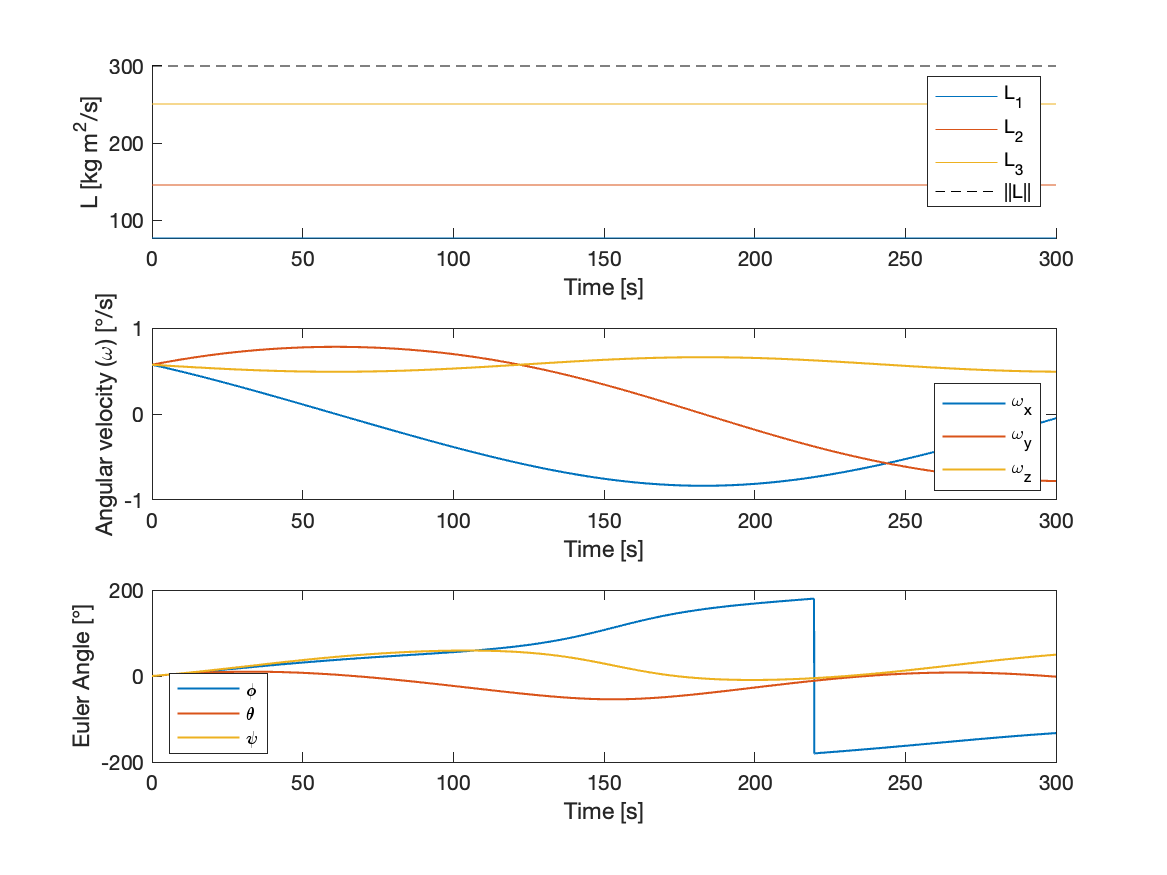
\includegraphics[scale=0.6]{Images/ps4_problem3b.png}
\caption{Angular momentum conserved with angular momentum components constant}
\label{fig:ps4_problem3b}
\end{figure}

\textit{c. Verify equilibrium and its stability similar to previous pset.}

By linearizing the Euler equations about equilibrium, the following result shows that periodic stability (in this case, about the z-axis) can be met with a reaction wheel if one of the following conditions are met:

\begin{align*}
    1)\; I_r \omega_r > (I_y - I_z) \omega_z \;\; AND \;\; I_r \omega_r > (I_x - I_z) \omega_z \\
    2)\; I_r \omega_r < (I_y - I_z) \omega_z \;\; AND \;\; I_r \omega_r < (I_x - I_z) \omega_z
\end{align*}

We demonstrate equilibrium and stability for this new system with the reaction wheel. Figures \ref{fig:ps4_problem3c_x.png}, \ref{fig:ps4_problem3c_y.png}, \ref{fig:ps4_problem3c_z.png} show the analysis for each of the principal axes. As before, the minimum and maximum inertia principal axes are periodically stable, but the intermediate axis is unstable.

This behavior resembles that found in Problem 2 above. In this case, we perturb each angular velocity as well as the rotor angular velocity. Our rotor velocity in this case is not enough to stabilize spin about the intermediate axis.

\begin{figure}[H]
\centering
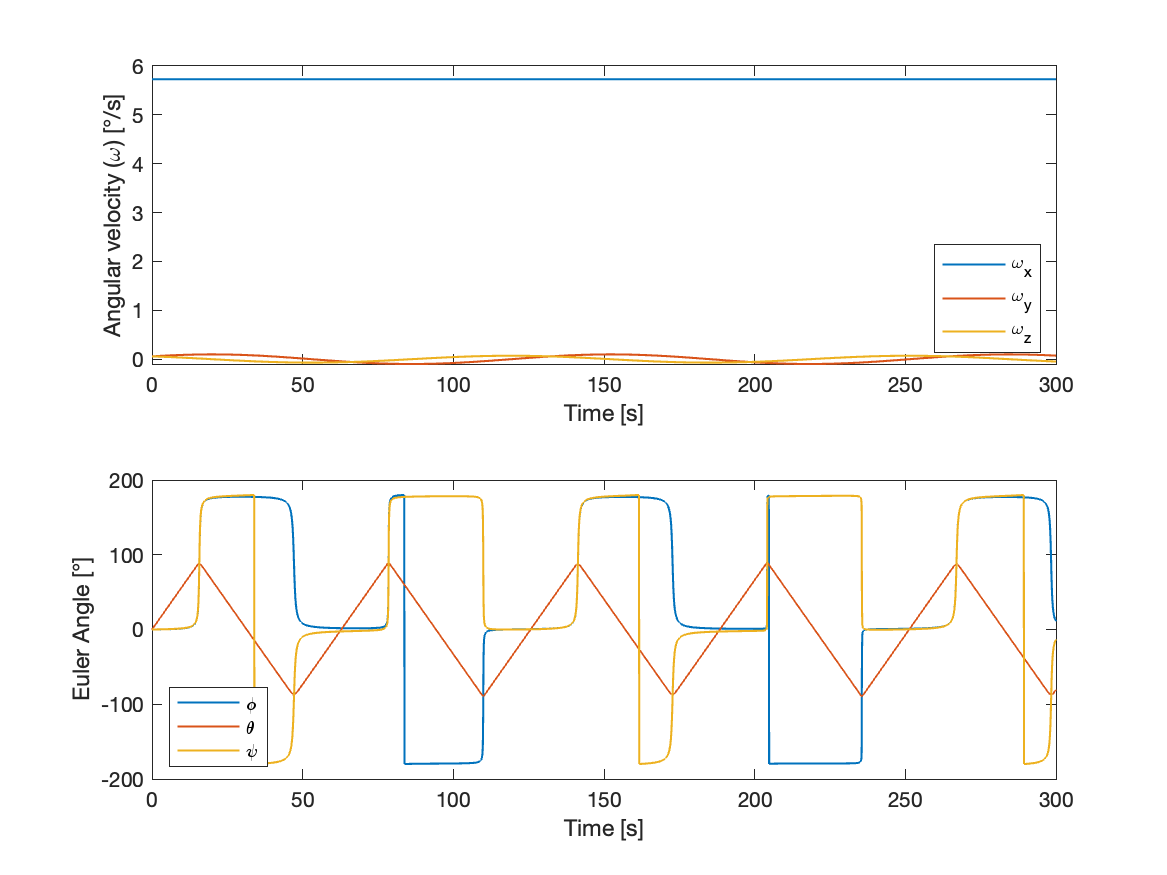
\includegraphics[scale=0.6]{Images/ps4_problem3c_x.png}
\caption{Stability analysis about minimum inertia principal axis}
\label{fig:ps4_problem3c_x.png}
\end{figure}

\begin{figure}[H]
\centering
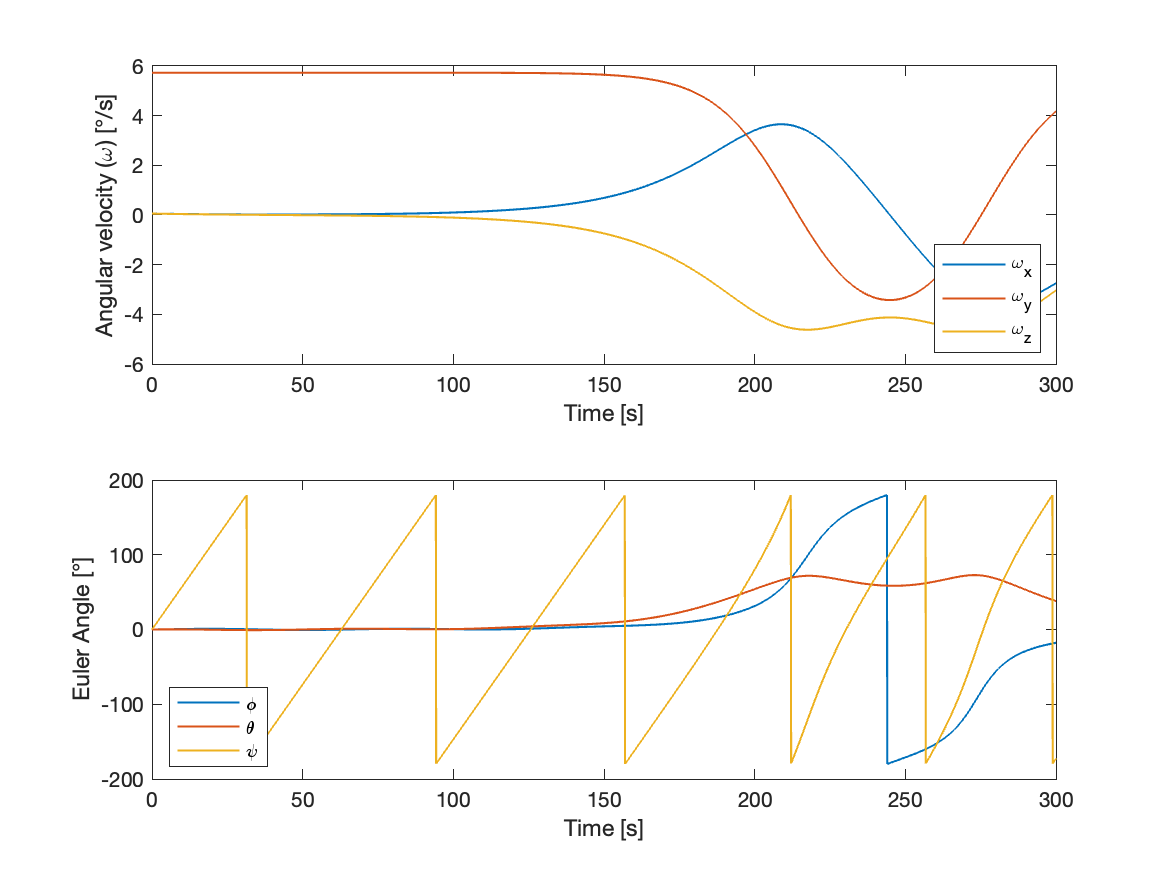
\includegraphics[scale=0.6]{Images/ps4_problem3c_y.png}
\caption{Stability analysis about intermediate axis}
\label{fig:ps4_problem3c_y.png}
\end{figure}

\begin{figure}[H]
\centering
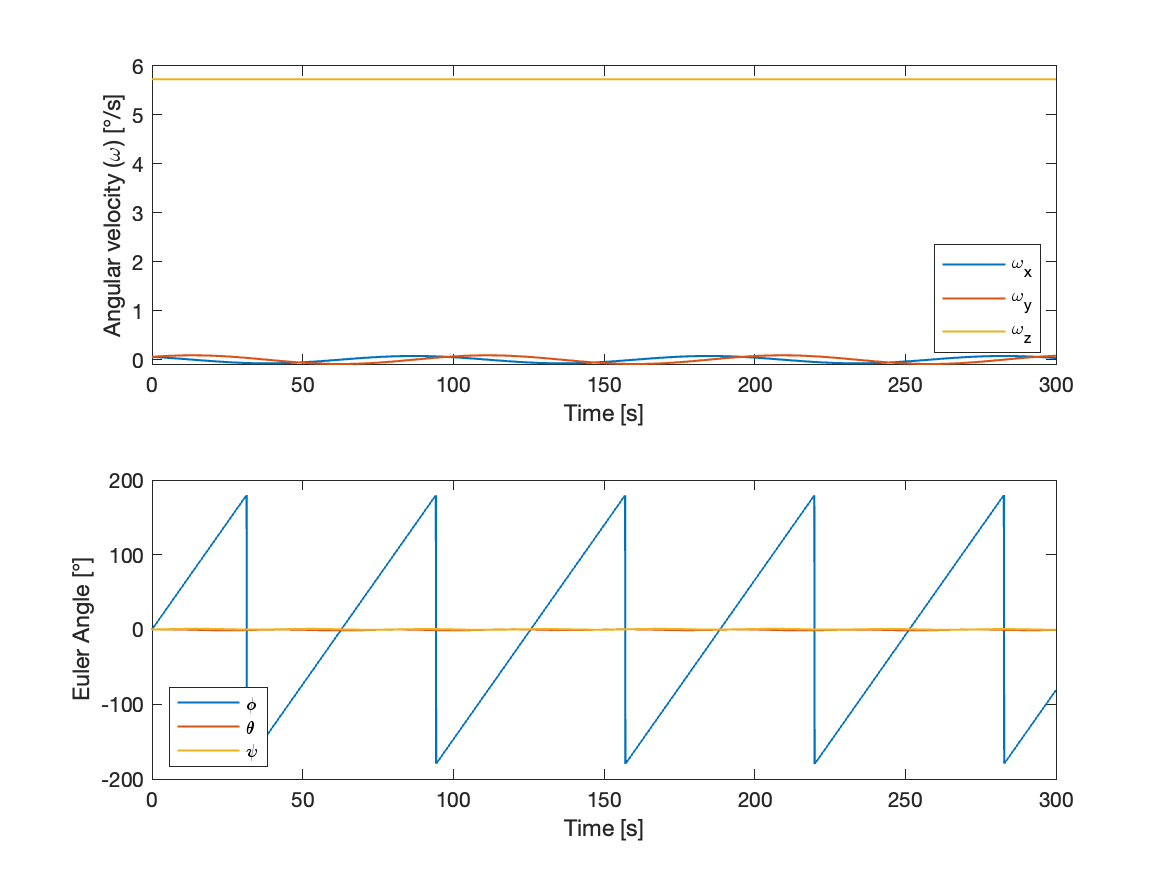
\includegraphics[scale=0.6]{Images/ps4_problem3c_z.png}
\caption{Stability analysis about maximum inertia principal axis}
\label{fig:ps4_problem3c_z.png}
\end{figure}

\newpage
\textit{d. Use the stability condition to make attitude motion stable for rotation about intermediate moment of inertia by changing moment of inertia and/or angular velocity of the momentum wheel or rotor.}

By increasing the angular velocity of the rotor by a factor of 10, we obtain a stable system for spin about the intermediate axes.

\begin{figure}[H]
\centering
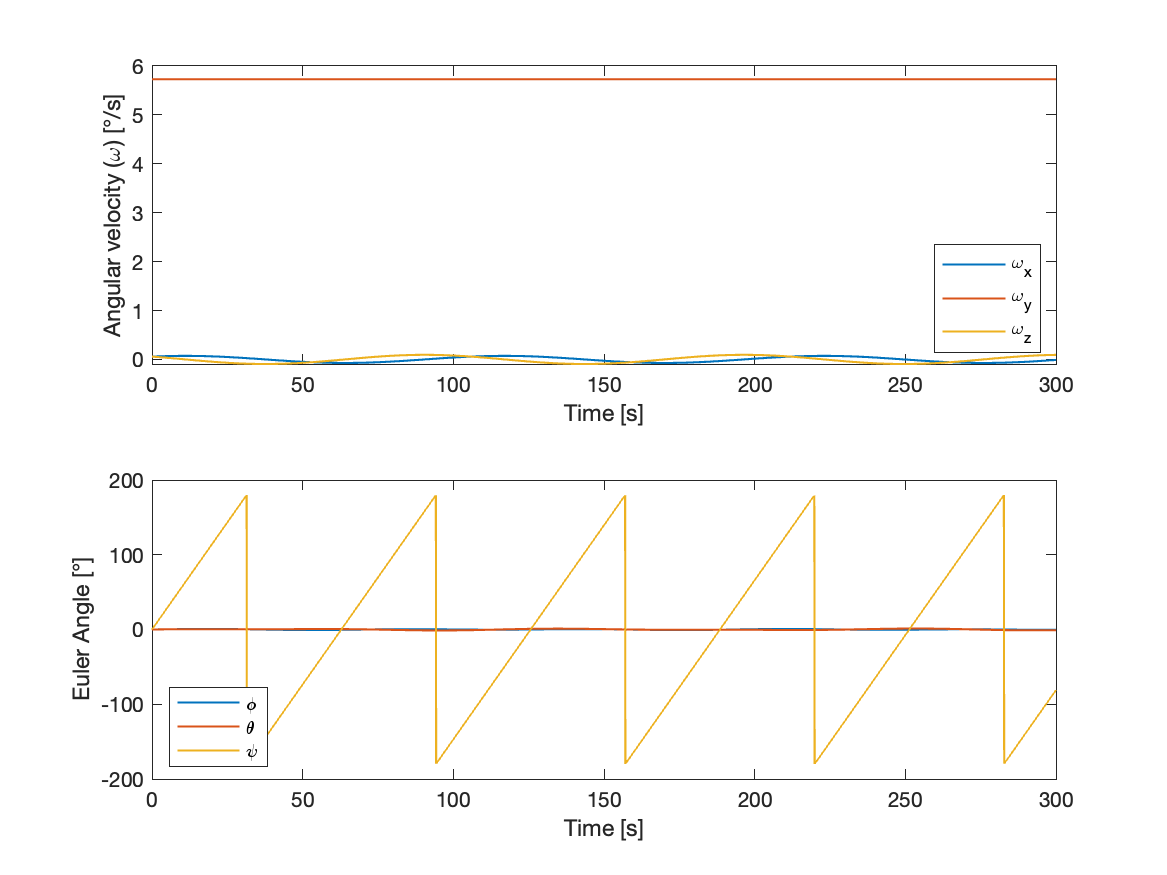
\includegraphics[scale=0.6]{Images/ps4_problem3d.png}
\caption{}
\label{fig:ps4_problem3d.png}
\end{figure}

\newpage
\textit{e. Try to make rotation about another arbitrary axis (potentially relevant to your project) stable through a generic momentum wheel or rotor.}

We choose to stabilize spin about the body x-axis, which is important for pointing our satellite and appropriately sweeping the target with our SAR. We use the rotation previously found between the principal and body axes to achieve this, applying the rotation to the angular velocity and the angular momentum vector direction of the momentum wheel.

\begin{figure}[H]
\centering
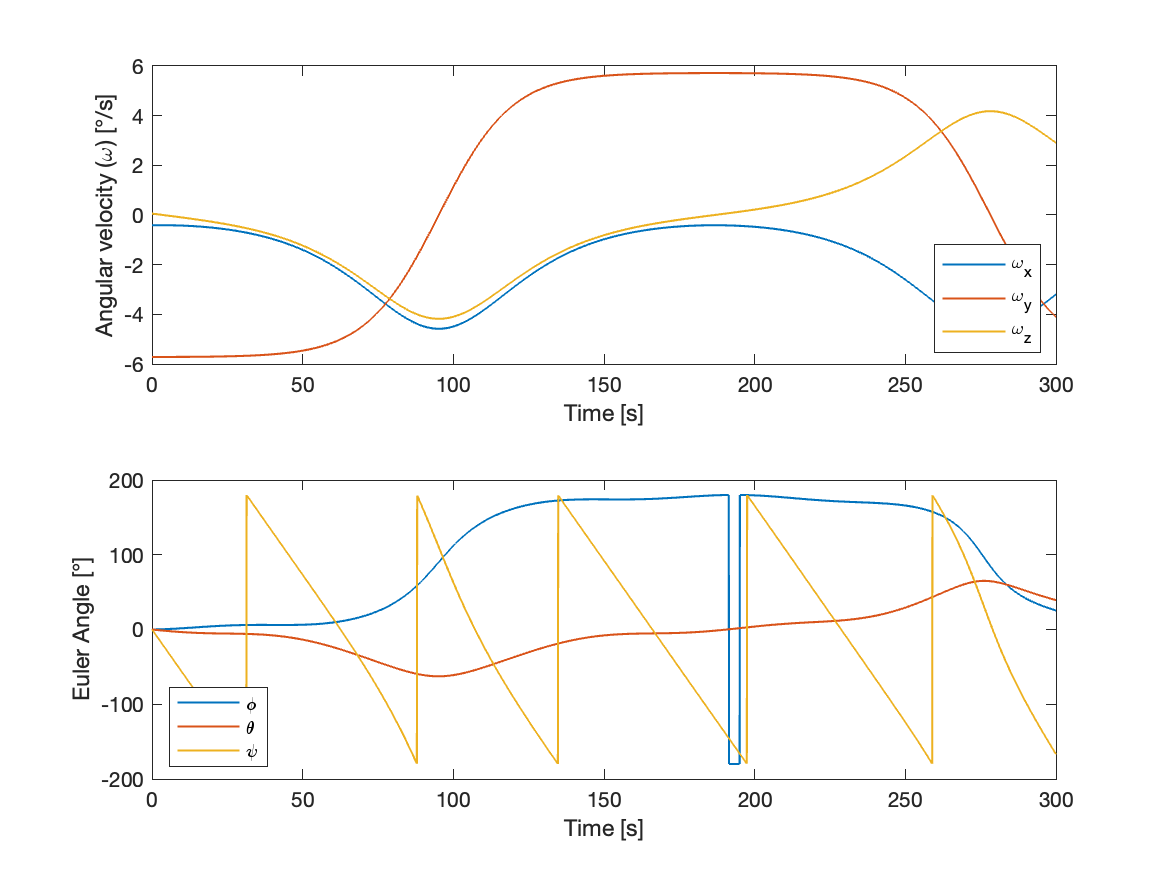
\includegraphics[scale=0.6]{Images/ps4_problem3e_unstable.png}
\caption{Initially unstable attitude with low momentum wheel angular velocity}
\label{fig:ps4_problem3e_unstable.png}
\end{figure}

\begin{figure}[H]
\centering
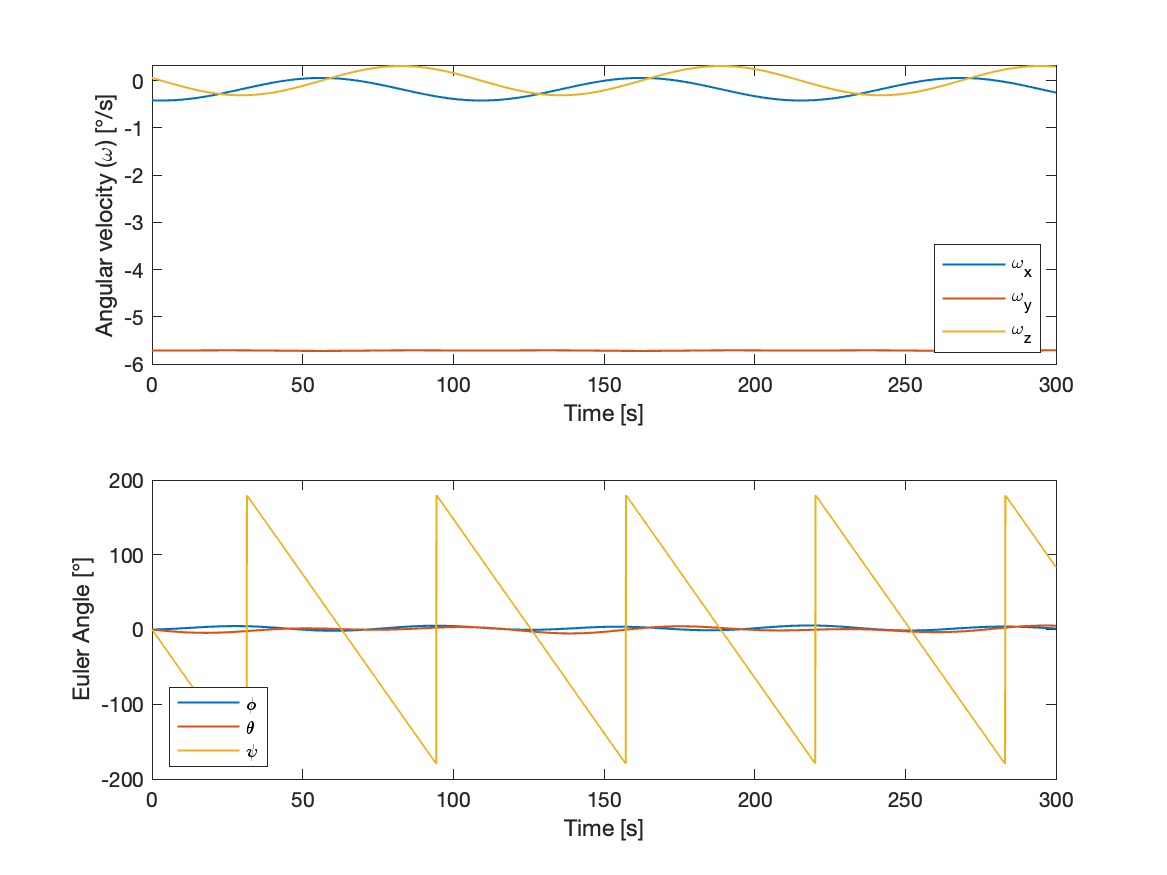
\includegraphics[scale=0.6]{Images/ps4_problem3e_stable.png}
\caption{Periodically stable attitude after increasing momentum wheel angular velocity 10x}
\label{fig:ps4_problem3e_stable.png}
\end{figure}

\subsection{PROBLEM 4}
\textit{Gravity gradient torque (modeling)}

\textit{a. Remove rotor.}

A new function was created without effect of the rotor.

\textit{b. Program gravity gradient torque. Feed torque to Euler equations. This is the first perturbation you model resulting from the interaction of the spacecraft with the environment. Hint: change your orbit to make gravity gradient significant if that’s not the case.}

The equations for the gravity gradient torque are below.

\begin{align*}
    I_x \dot{\omega_x} + (I_z - I_y) \omega_y \omega_z = 3 n^2 (I_z - I_y) c_y c_z \\
    I_y \dot{\omega_y} + (I_x - I_z) \omega_z \omega_x = 3 n^2 (I_x - I_z) c_z c_x \\
    I_z \dot{\omega_z} + (I_y - I_x) \omega_x \omega_y = 3 n^2 (I_y - I_x) c_x c_y \\
\end{align*}

In the above equation, $\Vec{c} = [c_x, c_y, c_z]^\intercal$ is the normalized direction of $\Vec{R}$.

The function \texttt{gravGrad} was developed to be used with \texttt{ode113} to propagate the Euler equations and kinematics with gravity gradient torques.

\lstinputlisting{src/gravGrad.m}

\textit{c. Verify that the magnitude of the modeled torque is consistent with the orbit and inertia tensor of your satellite. Hint: use simplified formulas from class on modeling of gravity gradient torque.}

We can estimate the order of magnitude for gravity gradient torques using the following equation.

\begin{align*}
    \Vec{M} &= \frac{3 \mu}{a^3}
    \begin{bmatrix}
    (I_z - I_y) c_y c_z \\
    (I_x - I_z) c_z c_x \\
    (I_y - I_x) c_x c_y
    \end{bmatrix}
\end{align*}

The parameters used were the known moments of inertia ($I_x = \qty{7707}{}$, $I_y = \qty{14563}{}$, $I_z = \qty{18050}{\kilogram\cdot\meter^2}$), known values for Earth ($a = \qty{7125.49}{km}$, $\mu = \qty{398600}{\km^3\per\second^2}$), and an arbitrary $\Vec{c} = [\frac{1}{\sqrt{3}}, \frac{1}{\sqrt{3}}, \frac{1}{\sqrt{3}}]$. With these values, we arrive at:

\begin{align*}
    \Vec{M} &=
\qty[parse-numbers = false]{
    \begin{bmatrix}
    0.384174 \\
    1.13956 \\
    -0.755387
    \end{bmatrix}
    \cdot
    10^{-2}
}{\newton\meter}
\end{align*}

These values are in line with what we see in Figure \ref{fig:ps4_problem4e_torque}.

\newpage
\textit{d. Numerically integrate Euler and Kinematic equations including gravity gradient from initial conditions corresponding to body axes aligned with the orbital frame (RTN). Verify that gravity gradient torque is zero, besides numerical errors. Hint: you may need to simplify the orbit to unperturbed circular to achieve this. Check that initial angular velocity matches mean motion.}

Figures \ref{fig:ps4_problem4d_torque}, \ref{fig:ps4_problem4d_angvel} demonstrate zero torque when aligned with RTN frame and constant angular velocity. Simulating for longer periods reveals the torque error is periodically stable.

\begin{figure}[H]
\centering
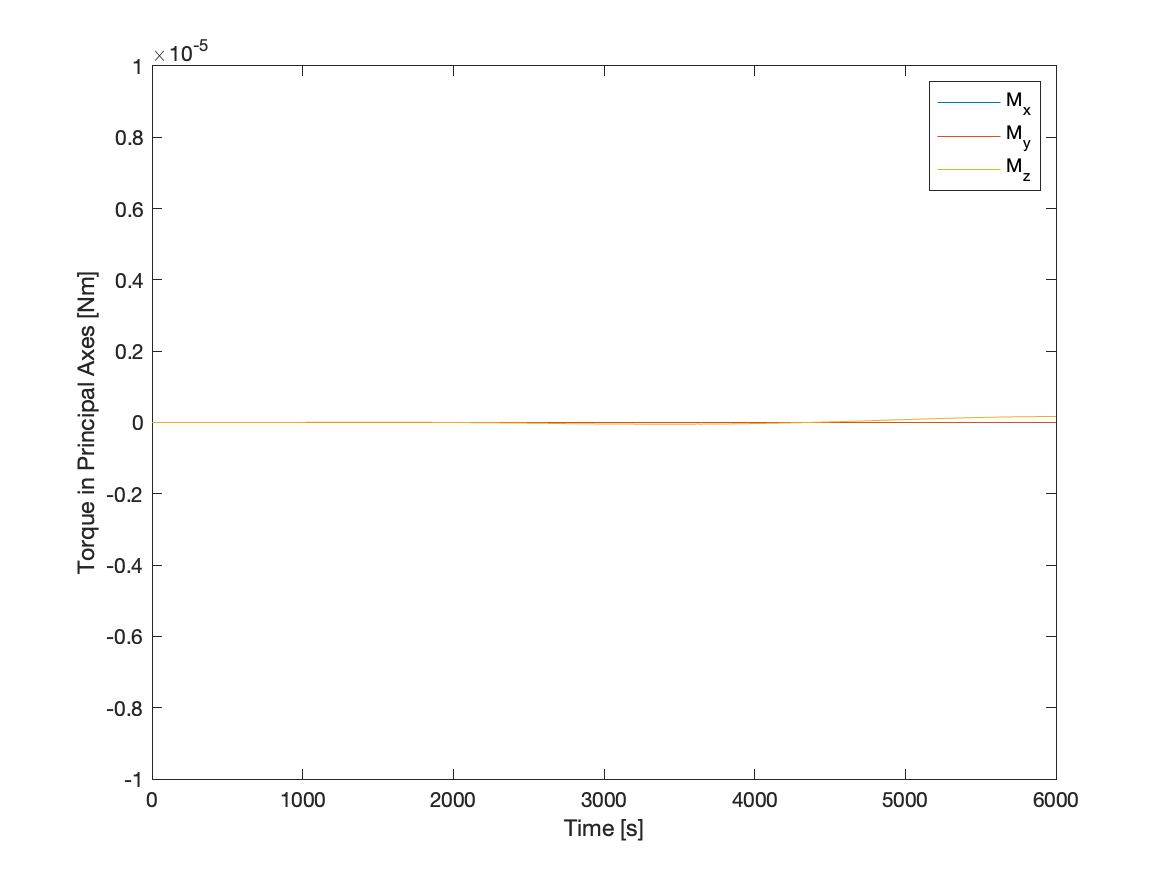
\includegraphics[scale=0.6]{Images/ps4_problem4d_torque.png}
\caption{Zero gravity gradient torque for satellite aligned with RTN frame}
\label{fig:ps4_problem4d_torque}
\end{figure}

\begin{figure}[H]
\centering
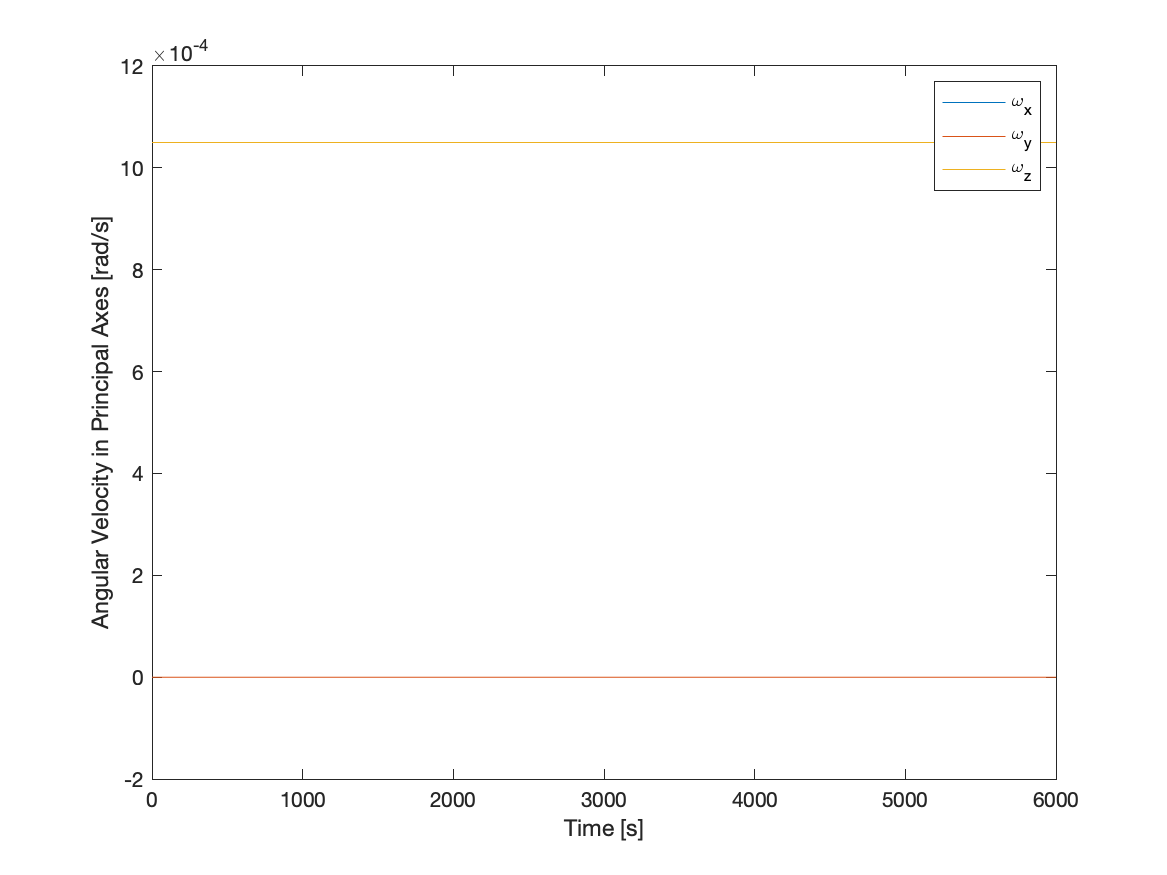
\includegraphics[scale=0.6]{Images/ps4_problem4d_angvel.png}
\caption{Angular velocity parallel to RTN normal equal to mean motion, all others zero}
\label{fig:ps4_problem4d_angvel}
\end{figure}

\textit{e. Numerically integrate Euler and Kinematic equations including gravity gradient from arbitrary initial conditions (e.g., relevant to your project). Plot external torque (3 components w.r.t. time) and resulting attitude motion (depends on attitude parameterization, add Euler angles for better geometrical interpretation) over multiple orbits. Comment on results.}

We choose initial conditions by aligning our body axes to RTN, which will more closely resemble the orientation of the satellite when collecting science data.

\begin{figure}[H]
\centering
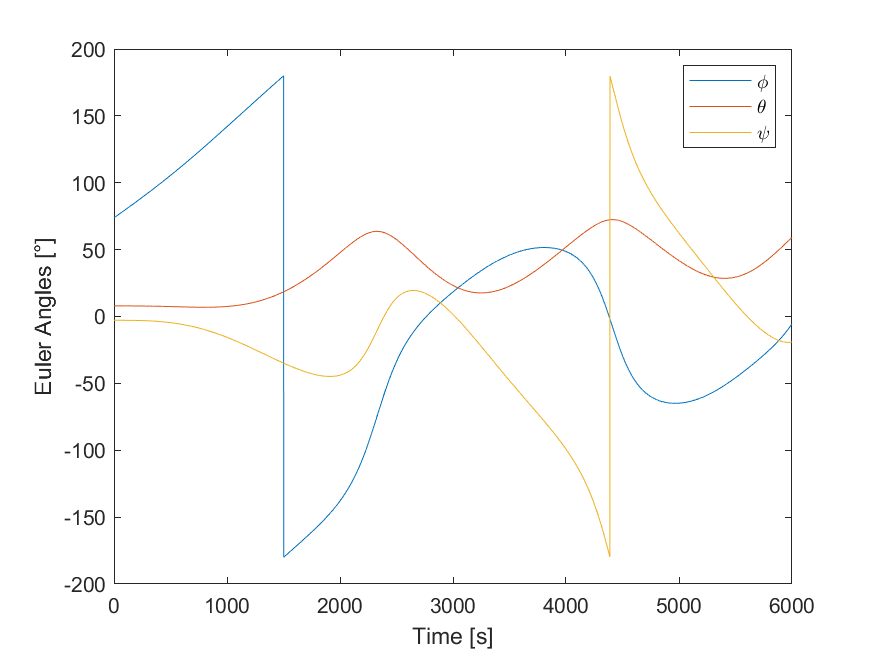
\includegraphics[scale=0.6]{Images/ps4_problem4e_angle.png}
\caption{Euler angles with gravity gradient for satellite with arbitrary initial conditions}
\label{fig:ps4_problem4e_angle}
\end{figure}

\begin{figure}[H]
\centering
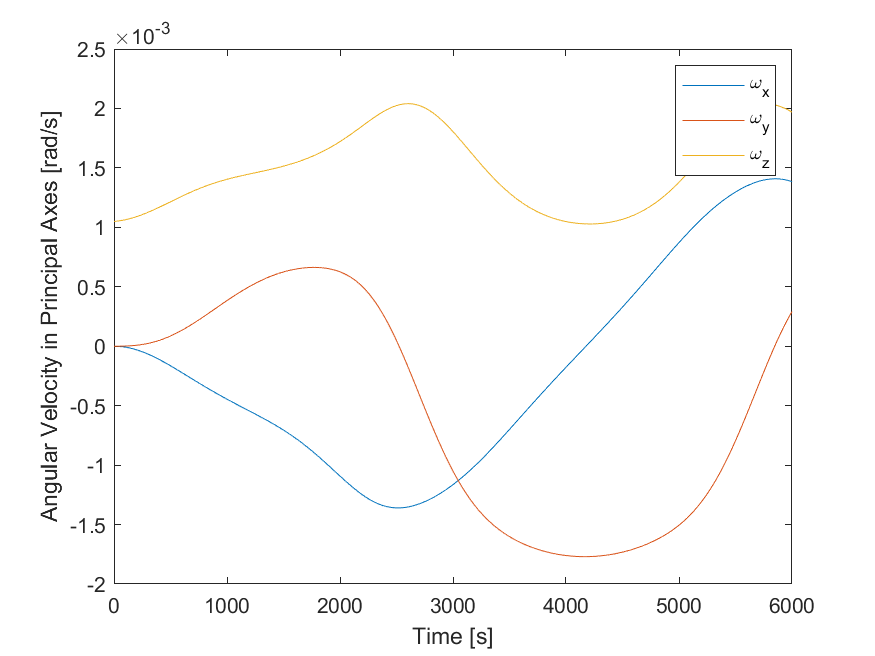
\includegraphics[scale=0.6]{Images/ps4_problem4e_angvel.png}
\caption{Angular velocity with gravity gradient for satellite with arbitrary initial conditions}
\label{fig:ps4_problem4e_angvel}
\end{figure}

The figures show that there is a noticeable effect of gravity gradient torque on the satellite, although the magnitude of the torque is low. This causes changes to our Euler angles throughout the orbit, meaning we will need a control system to stabilize and point our satellite in order to meet mission requirements.

\begin{figure}[H]
\centering
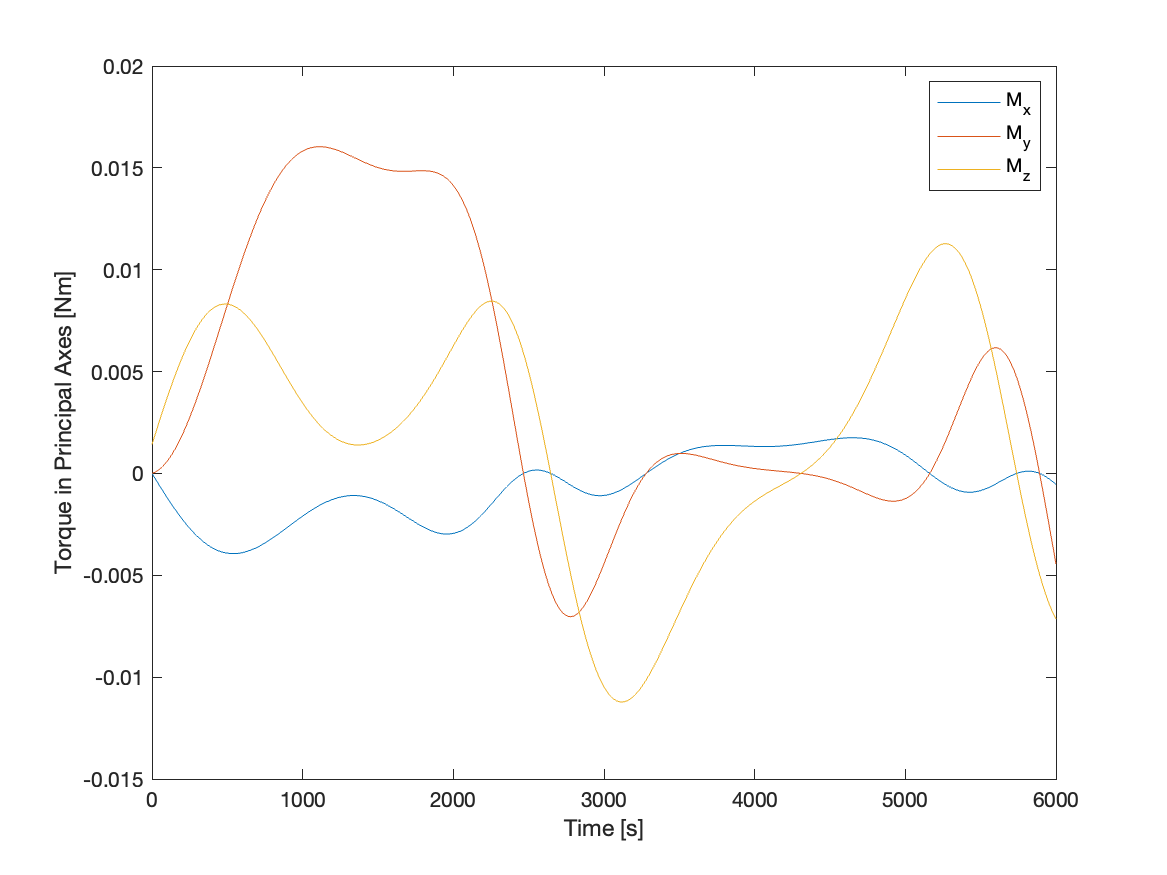
\includegraphics[scale=0.6]{Images/ps4_problem4e_torque.png}
\caption{Gravity gradient torques for satellite with arbitrary initial conditions}
\label{fig:ps4_problem4e_torque}
\end{figure}